
\chapter{Problems in two dimensions}

For two-dimensional equations, the domain is $\Omega \in \R^2$ and Sobolev space (\ref{sobolev_space}) becomes
\begin{align}
  \label{2d_sobolev_space}
  \mathcal{H}^1(\Omega) &= \left\{ u\ :\ \Omega \rightarrow \R\ \Bigg|\ u, \parder{u}{x}, \parder{u}{y} \in L^2(\Omega) \right\}.
\end{align}
The two-dimensional domain is discretized into either triangular or quadrilateral elements, with new interpolation functions that satisfy a two-dimensional analog of interpolation properties (\ref{interpolation_properties}).  For an excellent explanation of the resulting 2D Galerkin system analogous to (\ref{intro_galerkin_system}), see \citet{elman_2005}.

In this chapter, we solve the two-dimensional variant of heat equation (\ref{intro_ode}) and the Stokes equations.

%===============================================================================

\section{Poisson equation}

\index{Linear differential equations!2D}
\index{Poisson equation}
The Poisson equation to be solved over the domain $\Omega = [0,1] \times [0,1]$ is
\begin{align}
  \label{2d_poisson_start}
  -\nabla^2 u &= f &&\text{ in } \Omega \\
  f &= 10 \sin\left(\frac{2\pi x}{L}\right) \sin\left(\frac{2\pi y}{L}\right) &&\text{ in } \Omega \\
  \nabla u \cdot \normal &= g_N = \sin(x) &&\text{ on } \Gamma_N, \Gamma_S \\
  \label{2d_poisson_end}
  u &= g_D = 1 &&\text{ on } \Gamma_E, \Gamma_W,
\end{align}
where $\Gamma_N$, $\Gamma_S$, $\Gamma_E$, and $\Gamma_W$ are the North, South, East and West boundaries, $L=1$ is the length of the square side, and $\normal$ is the outward normal to the boundary $\Gamma$.

The associated Galerkin weak form with test function $\phi \in \testspace$ defined by (\ref{test_space}) is
\begin{align*}
  -\int_{\Omega} \nabla^2 u \phi \d{\Omega} &= \int_{\Omega} f \phi \d{\Omega} \\
  \int_{\Omega} \nabla u \cdot \nabla \phi \d{\Omega} - \int_{\Gamma} \phi \nabla u \cdot \normal \d{\Gamma} &= \int_{\Omega} f \phi \d{\Omega} \\
  \int_{\Omega} \nabla u \cdot \nabla \phi \d{\Omega} - \int_{\Gamma_N} \phi g_N \d{\Gamma_N} - \int_{\Gamma_S} \phi g_N \d{\Gamma_S} &= \int_{\Omega} f \phi \d{\Omega},
\end{align*}
and so the variational problem consists of finding $u \in \trialspace$ (see trial space \ref{trial_space}) such that
\begin{align*}
  a(u,\phi) &= L(\phi) && \forall \phi \in S_0^h \subset \mathcal{H}_{E_0}^1(\Omega),
\end{align*}
subject to Dirichlet condition (\ref{2d_poisson_end}), where
\begin{align*}
  L(\phi) &= \int_{\Gamma_N} \phi g_N \d{\Gamma_N} + \int_{\Gamma_S} \phi g_N \d{\Gamma_S} + \int_{\Omega} f \phi \d{\Omega}, \\
  a(u,\phi) &= \int_{\Omega} \nabla u \cdot \nabla \phi \d{\Omega}.
\end{align*}
This form is all that is required to derive an approximate solution with FEniCS, as demonstrated by Code Listing \ref{2d_poisson_code} and Figure \ref{2d_poisson_image}.

\pythonexternal[label=2d_poisson_code, caption={FEniCS solution to two-dimensionial Poisson problem (\ref{2d_poisson_start} -- \ref{2d_poisson_end}).}]{scripts/fenics_intro/2D_poisson.py}

\begin{figure}
  \centering
    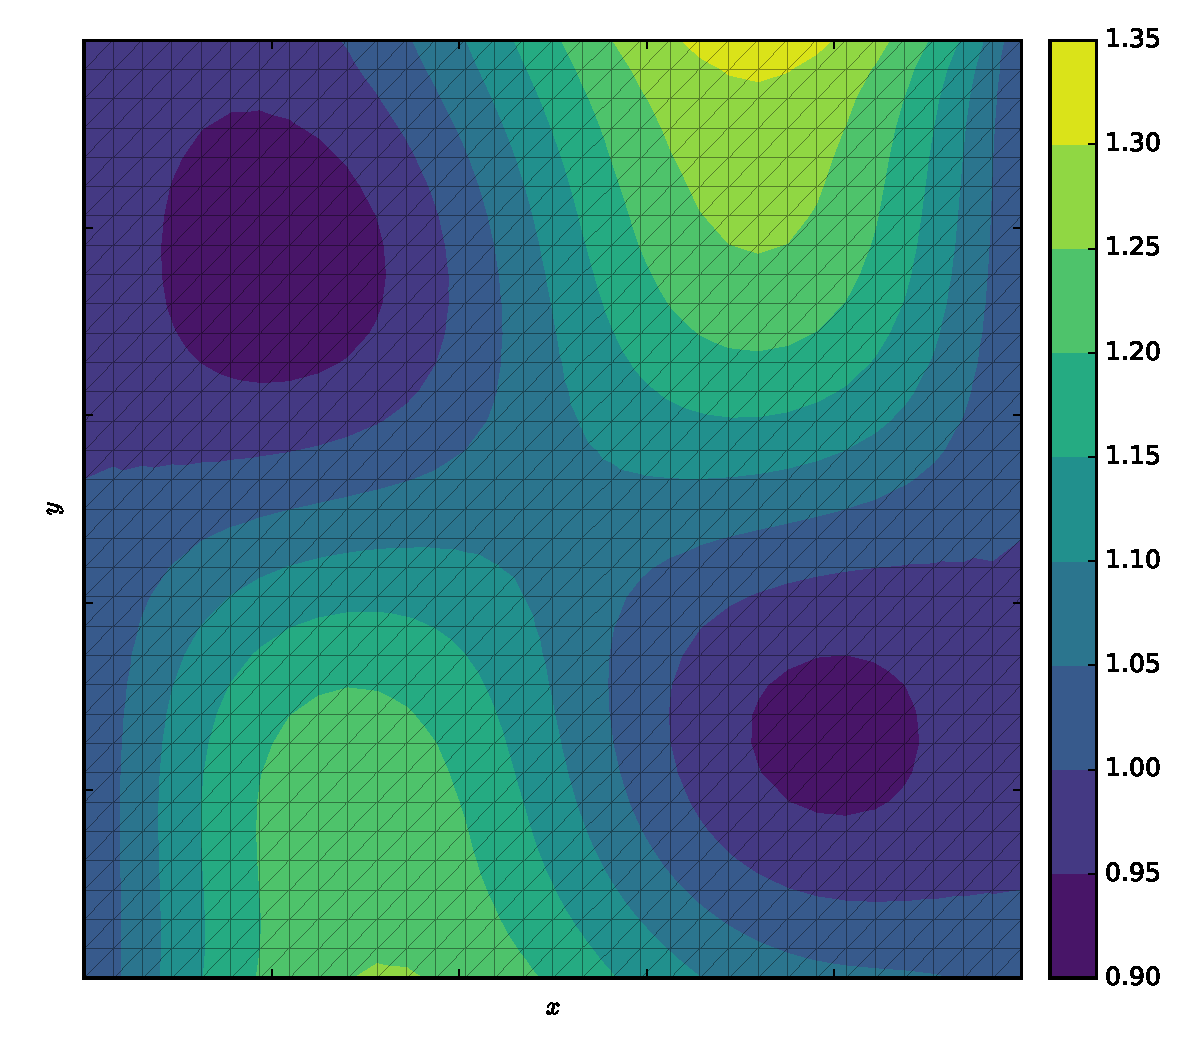
\includegraphics[width=\linewidth]{images/fenics_intro/2Dpoisson.pdf}
  \caption[Two-dimension Poisson example]{Poisson solution for a uniform $32 \times 32$ node mesh.}
  \label{2d_poisson_image}
\end{figure}

%===============================================================================

\section{Stokes equations with no-slip boundary conditions} \label{ssn_intro_stokes_2d}

\index{Linear differential equations!2D}
\index{Stokes equations!No-slip}
The Stokes equations for incompressible fluid over the domain $\Omega = [0,1] \times [0,1]$ are
\begin{align}
  \label{intro_stokes_momentum}
  -\nabla \cdot \ranktwo{\sigma} &= \rankone{f} &&\text{ in } \Omega &&\leftarrow \text{ conservation of momentum} \\
  \label{intro_stokes_mass}
  \nabla \cdot \rankone{u} &= 0 &&\text{ in } \Omega &&\leftarrow \text{ conservation of mass},
\end{align}
where $\ranktwo{\sigma}$ is the Cauchy-stress tensor defined as $\ranktwo{\sigma} = 2\eta \ranktwo{\dot{\epsilon}} - p\ranktwo{I}$; viscosity $\eta$, strain-rate tensor
\begin{align}
  \label{intro_strain_rate_tensor}
  \ranktwo{\dot{\epsilon}} &= \frac{1}{2}\left[\nabla \rankone{u} + (\nabla \rankone{u})\T \right] \notag \\
  &= \begin{bmatrix}
       \parder{u}{x} & \frac{1}{2} \left( \parder{u}{y} + \parder{v}{x} \right) \\
       \frac{1}{2} \left( \parder{v}{x} + \parder{u}{y} \right) & \parder{v}{y}
     \end{bmatrix};
\end{align}
velocity $\rankone{u}$ with components $u$, $v$ in the $x$ and $y$ directions, and pressure $p$; and vector of internal forces $\rankone{f}$.  For our example, we take $\rankone{f}=\rankone{0}$ and boundary conditions
\begin{align}
  \label{intro_stokes_gD_N_S_D}
  \rankone{u} &= \rankone{g_D} = \rankone{0} &&\text{ on } \Gamma_N, \Gamma_S, \Gamma_D \\
  \label{intro_stokes_gD_E}
  \rankone{u} &= \rankone{g_D} = [-\sin(\pi y)\ 0]\T &&\text{ on } \Gamma_E \\
  \label{intro_stokes_gN}
  \ranktwo{\sigma} \cdot \normal &= \rankone{g_N} = [g_{N_x}\ g_{N_y}]\T = \rankone{0} &&\text{ on } \Gamma_W,
\end{align}
where $\Gamma_E$, $\Gamma_W$, $\Gamma_N$, and $\Gamma_S$ are the East, West, North, and South boundaries, $\Gamma_D$ is the dolphin boundary (Figure \ref{intro_stokes_2d}) and $\normal$ is the outward-pointing normal vector to these faces. For obvious reasons, velocity boundary condition (\ref{intro_stokes_gD_N_S_D}) is referred to as a \emph{no-slip} boundary.

It may be of interest to see how the conservation of momentum equations look in their expanded form,
\begin{align*}
  -\nabla \cdot \ranktwo{\sigma} &= \rankone{f} \\
  \begin{bmatrix}
    \parder{\sigma_{xx}}{x} + \parder{\sigma_{xy}}{y} \\ 
    \parder{\sigma_{yx}}{x} + \parder{\sigma_{yy}}{y} \\ 
  \end{bmatrix} &=
  \begin{bmatrix}
    0 \\ 0
  \end{bmatrix},
\end{align*}
providing two equations,
\begin{align*}
    \parder{}{x} \left[2\eta \parder{u}{x} \right]  - \parder{p}{x} + \parder{}{y} \left[\eta \left( \parder{u}{x} + \parder{v}{y} \right) \right] &= 0 \\ 
    \parder{}{x} \left[\eta \left( \parder{v}{y} + \parder{u}{x} \right) \right]  + \parder{}{y} \left[2\eta \parder{v}{y} \right] - \parder{p}{y} &= 0, 
\end{align*}
which along with conservation of mass equation (\ref{intro_stokes_mass}), also referred to as the \emph{incompressibility constraint}
\begin{align*}
  \nabla \cdot \rankone{u} &= \parder{u}{x} + \parder{v}{y} = 0, 
\end{align*}
makes three equations with three unknowns $u$, $v$, and $p$.

Neumann condition (\ref{intro_stokes_gN}) may be expanded into
\begin{align}
  \label{intro_stokes_outflow}
  2 \eta \dot{\epsilon}_{xx} n_x - p n_x + 2 \eta \dot{\epsilon}_{xy} n_y &= g_{N_x} \\
  2 \eta \dot{\epsilon}_{yx} n_x + 2 \eta \dot{\epsilon}_{yy} n_y - p n_y &= g_{N_y}.
\end{align}
The pressure boundary condition on the outflow boundary $\Gamma_W$ may be discovered by integrating boundary condition (\ref{intro_stokes_outflow}) along $\Gamma_W$ with $\normal = [-1\ 0]\T$, assuming a constant viscosity $\eta$, and strain-rate tensor definition (\ref{intro_strain_rate_tensor}),
\begin{align*}
  - 2 \eta \int_{\Gamma_W} \parder{u}{x} \d{\Gamma_W} + \int_{\Gamma_W} p \d{\Gamma_W} &= \int_{\Gamma_W} g_{N_x} \d{\Gamma_W}.
\end{align*}
Next, constraint (\ref{intro_stokes_mass}) implies that $\partial_x u = - \partial_y v$ and thus
\begin{align*}
  2 \eta \int_0^1 \parder{v}{y} \d{y} + \int_0^1 p \d{y} &= \int_{\Gamma_W} g_{N_x} \d{\Gamma_W} \\
  2 \eta v(0,1) - 2 \eta v(0,0) + \int_0^1 p \d{y} &= \int_{\Gamma_W} g_{N_x} \d{\Gamma_W} \\
  \int_0^1 p \d{y} &= \int_{\Gamma_W} 0 \d{\Gamma_W},
\end{align*}
which implies that $p = 0$ over the entire outflow boundary $\Gamma_W$ (for further illustration, see \citet{elman_2005}).

The weak form for problem (\ref{intro_stokes_momentum}, \ref{intro_stokes_mass}, \ref{intro_stokes_gD_N_S_D} -- \ref{intro_stokes_gN}) is formed by taking the inner product of both sides of the conservation of momentum equation with the vector test function $\rankone{\Phi} = [\phi\ \psi ]\T \in \rankone{S_0^h} \subset \left( \mathcal{H}_{E_0}^1(\Omega) \right)^2$ (see test space (\ref{test_space})) integrating over the domain $\Omega$,
\begin{align*}
  -\int_{\Omega} \nabla \cdot \ranktwo{\sigma} \cdot \rankone{\Phi} \d{\Omega} &= \int_{\Omega} \rankone{f} \cdot \rankone{\Phi} \d{\Omega},
\end{align*}
then integrate by parts to get 
\begin{align*}
  \int_{\Omega} \ranktwo{\sigma} : \nabla \rankone{\Phi} \d{\Omega} - \int_{\Gamma} \ranktwo{\sigma} \cdot \normal \cdot \rankone{\Phi} \d{\Gamma} &= \int_{\Omega} \rankone{f} \cdot \rankone{\Phi} \d{\Omega} \\
  \int_{\Omega} \ranktwo{\sigma} : \nabla \rankone{\Phi} \d{\Omega} &= \int_{\Omega} \rankone{f} \cdot \rankone{\Phi} \d{\Omega},
\end{align*}
where the facts that $\ranktwo{\sigma} \cdot \normal = \rankone{0}$ on the West boundary and Dirichlet conditions exist on the North, South, East, and dolphin boundaries has been used.  Next, taking the inner product of incompressibility (conservation of mass) equation (\ref{intro_stokes_mass}) with the test function $\xi \in M^h \subset L^2(\Omega)$ (see $L^2$ space (\ref{l2_space})) integrating over $\Omega$,
\begin{align*}
  \int_{\Omega} \left( \nabla \cdot \rankone{u} \right) \xi \d{\Omega} &= 0.
\end{align*}

Finally, using the fact that the right-hand side of incompressibility equation (\ref{intro_stokes_mass}) is zero, the \index{Mixed methods} \emph{mixed formulation} (see for example \citet{johnson_2009}) consists of finding \emph{mixed approximation} $\rankone{u} \in \rankone{S_E^h} \subset \left( \mathcal{H}_E^1(\Omega) \right)^2$ and $p \in M^h \subset L^2(\Omega)$ such that
{\scriptsize
\begin{align}
  \label{intro_stokes_mixed_problem}
  a(\rankone{u},p,\rankone{\Phi},\xi) &= L(\rankone{\Phi}) && \forall \rankone{\Phi} \in \rankone{S_0^h} \subset \left( \mathcal{H}_{E_0}^1(\Omega) \right)^2,\ \xi \in M^h \subset L^2(\Omega),
\end{align}}
subject to Dirichlet conditions (\ref{intro_stokes_gD_N_S_D} -- \ref{intro_stokes_gN}) and
\begin{align*}
  a(\rankone{u},p,\rankone{\Phi},\xi) &= \int_{\Omega} \ranktwo{\sigma} : \nabla \rankone{\Phi} \d{\Omega} + \int_{\Omega} \left( \nabla \cdot \rankone{u} \right) \xi \d{\Omega}, \\
  L(\rankone{\Phi}) &= \int_{\Omega} \rankone{f} \cdot \rankone{\Phi} \d{\Omega}.
\end{align*}

\subsection{Stability}

\index{Stokes equations!Stability}
In order to derive a unique solution for pressure $p$, the trial and test spaces must be chosen in such a way that the \emph{inf-sup condition}
\begin{align}
  \label{inf_sup_condition}
  \min_{\xi \neq \text{constant}} \left\{ \max_{\rankone{\Phi} \neq \rankone{0}} \left\{ \frac{\left| \left( \xi, \nabla \cdot \rankone{\Phi} \right) \right|}{\Vert \rankone{\Phi} \Vert_{1,\Omega} \Vert \xi \Vert_{0,\Omega} } \right\} \right\} \geq \gamma
\end{align}
is satisfied for any conceivable grid and some constant $\gamma$ \citep{elman_2005}.  The notation $(f,g) = \int_{\Omega} f g \d{\Omega}$ is the inner product, $\Vert \rankone{f} \Vert_{1,\Omega} = \left( \int_{\Omega} \left[ \rankone{f} \cdot \rankone{f} + \nabla \rankone{f} : \nabla \rankone{f} \right] \d{\Omega} \right)^{\nicefrac{1}{2}}$ is the $\rankone{S_E^h}$-norm, and $\Vert f \Vert_{0,\Omega} = \Vert f - \frac{1}{|\Omega|} \int_{\Omega} f \d{\Omega} \Vert$ is a so-called \emph{quotient space norm} \citep{elman_2005}.

One way of satisfying inf-sup condition (\ref{inf_sup_condition}) is through the use of Taylor-Hood finite element space \citep{taylor_1973}, which utilize a quadratic function space for the velocity vector components and the linear Lagrange function space for the pressure.

The velocity and pressure solutions to (\ref{intro_stokes_mixed_problem}) using Taylor-Hood elements are depicted in Figure \ref{intro_stokes_2d} and generated by Code Listing \ref{2d_stokes_no_slip_code}.

\section{Stokes equations with Navier boundary conditions} \label{ssn_intro_stokes_2d_slip}

\index{Linear differential equations!2D}
\index{Stokes equations!Navier boundary conditions}
The \emph{Navier} boundary conditions \citep{navier_1823}---referred to also as slip-friction boudnary conditions---for Stokes equations (\ref{intro_stokes_momentum}, \ref{intro_stokes_mass}) using an identical domain $\Omega$ as in \S \ref{ssn_intro_stokes_2d} may be generated by replacing no-slip boundary condition (\ref{intro_stokes_gD_N_S_D}) with the pair of boundary conditions
\begin{align}
  \label{intro_stokes_gD_N_S_D_slip}
  \rankone{u} \cdot \normal &= g_D = 0 &&\text{ on } \Gamma_N, \Gamma_S, \Gamma_D \\
  \label{intro_stokes_gN_N_S_D_fric}
  \left( \ranktwo{\sigma} \cdot \normal \right)_{\Vert} &= \rankone{g_N} = -\beta \rankone{u} &&\text{ on } \Gamma_N, \Gamma_S, \Gamma_D,
\end{align}
where $(\rankone{v})_{\Vert} = \rankone{v} - \left( \rankone{v} \cdot \normal \right) \normal$ denotes the tangential component of a vector $\rankone{v}$ and $\beta \geq 0$ is a friction coefficient.  Boundary conditions (\ref{intro_stokes_gD_N_S_D_slip}, \ref{intro_stokes_gN_N_S_D_fric}) are equivalent to no-slip boundary condition (\ref{intro_stokes_gD_N_S_D}) as $\beta$ approaches infinity.  Note also that impenetrability condition (\ref{intro_stokes_gD_N_S_D_slip}) specifies one component of velocity and is an essential boundary condition, while friction condition (\ref{intro_stokes_gN_N_S_D_fric}) specifies the other component (in three dimension it would specify the other two components) and is a natural boundary condition.  For comparison purposes, we use the same inflow boundary condition (\ref{intro_stokes_gD_E}) and outflow boundary condition (\ref{intro_stokes_gN}).

The weak form for problem (\ref{intro_stokes_momentum}, \ref{intro_stokes_mass}, \ref{intro_stokes_gD_N_S_D_slip}, \ref{intro_stokes_gN_N_S_D_fric}, \ref{intro_stokes_gD_E} \ref{intro_stokes_gN}) is formed by taking the inner product of both sides of the conservation of momentum equation with the vector test function $\rankone{\Phi} = [\phi\ \psi ]\T \in \rankone{S_0^h} \subset \left( \mathcal{H}_{E_0}^1(\Omega) \right)^2$ (see test space (\ref{test_space})) integrating over the domain $\Omega$,
\begin{align*}
  -\int_{\Omega} \nabla \cdot \ranktwo{\sigma} \cdot \rankone{\Phi} \d{\Omega} &= \int_{\Omega} \rankone{f} \cdot \rankone{\Phi} \d{\Omega},
\end{align*}
then integrate by parts to get and add the incompressibility constraint as performed in \S \ref{ssn_intro_stokes_2d},
{\footnotesize
\begin{align}
  \label{intro_stokes_slip_first_var_form}
  \int_{\Omega} \ranktwo{\sigma} : \nabla \rankone{\Phi} \d{\Omega} - \int_{\Gamma} \ranktwo{\sigma} \cdot \normal \cdot \rankone{\Phi} \d{\Gamma} + \int_{\Omega} \left( \nabla \cdot \rankone{u} \right) \xi \d{\Omega} &= \int_{\Omega} \rankone{f} \cdot \rankone{\Phi} \d{\Omega}.
\end{align}}
Expanding tangential stress condition (\ref{intro_stokes_gN_N_S_D_fric}), we have
\begin{align*}
  \ranktwo{\sigma} \cdot \normal &= \left( \normal \cdot \ranktwo{\sigma} \cdot \normal \right) \normal - \beta \rankone{u},
\end{align*}
producing
\begin{align}
  \label{intro_stokes_slip_intermediate_var_form}
  \mathcal{B}_{\Omega} + \mathcal{B}_{\Gamma_G} + \mathcal{B}_{\Gamma_E} = \mathcal{F}
\end{align}
with individual terms
\begin{align*}
  \mathcal{B}_{\Omega} &= + \int_{\Omega} \ranktwo{\sigma}(\rankone{u},p) : \nabla \rankone{\Phi} \d{\Omega} + \int_{\Omega} \left( \nabla \cdot \rankone{u} \right) \xi \d{\Omega} \\
  \mathcal{B}_{\Gamma_G} &= - \int_{\Gamma_G} \left( \normal \cdot \ranktwo{\sigma}(\rankone{u},p) \cdot \normal \right) \normal \cdot \rankone{\Phi} \d{\Gamma_G} + \int_{\Gamma_G} \beta \rankone{u} \cdot \rankone{\Phi} \d{\Gamma_G} \\
  \mathcal{B}_{\Gamma_E} &= - \int_{\Gamma_E} \ranktwo{\sigma}(\rankone{u},p) \cdot \normal \cdot \rankone{\Phi} \d{\Gamma_E} \\
  \mathcal{F} &= + \int_{\Omega} \rankone{f} \cdot \rankone{\Phi} \d{\Omega}, 
\end{align*}
where $\Gamma_G = \Gamma_N \cup \Gamma_S \cup \Gamma_D$ is the entire slip-friction boundary, and the fact that $\ranktwo{\sigma} \cdot \normal = \rankone{0}$ on the West boundary $\Gamma_W$ has been used.

A method devised by \index{Nitsche method} \citet{nitsche_1970/71} and further explained by \citet{freund_1995} imposes Dirichlet conditions (\ref{intro_stokes_gD_E}, \ref{intro_stokes_gD_N_S_D_slip}) in a weak form by adjoining symmetric terms to (\ref{intro_stokes_slip_intermediate_var_form}),
\begin{align}
  \label{intro_stokes_slip_var_form}
  \mathcal{B}_{\Omega} + \mathcal{B}_{\Gamma_G} + \mathcal{B}_{\Gamma_G}^W + \mathcal{B}_{\Gamma_E} + \mathcal{B}_{\Gamma_E}^W = \mathcal{F} + \mathcal{F}^W,
\end{align}
where
{\footnotesize
\begin{align*}
  \mathcal{B}_{\Gamma_G}^W = &- \int_{\Gamma_G} \left( \normal \cdot \ranktwo{\sigma}(\rankone{\Phi},\xi) \cdot \normal \right) \normal \cdot \rankone{u}  \d{\Gamma_G} + \gamma \int_{\Gamma_G} \frac{1}{h} \left( \rankone{u} \cdot \normal \right) \left( \rankone{\Phi} \cdot \normal \right) \d{\Gamma_G} \\
  \mathcal{B}_{\Gamma_E}^W = &- \int_{\Gamma_E} \ranktwo{\sigma}(\rankone{\Phi},\xi) \cdot \normal \cdot \rankone{u} \d{\Gamma_E} + \gamma \int_{\Gamma_E} \frac{1}{h} \left( \rankone{\Phi} \cdot \rankone{u} \right) \d{\Gamma_E} \\
  \mathcal{F}^W = &- \int_{\Gamma_G} \left( \normal \cdot \ranktwo{\sigma}(\rankone{\Phi},\xi) \cdot \normal \right) g_D \d{\Gamma_G} + \gamma \int_{\Gamma_G} \frac{1}{h} g_D \rankone{\Phi} \cdot \normal \d{\Gamma_G} \\
  &- \int_{\Gamma_E} \ranktwo{\sigma}(\rankone{\Phi},\xi) \cdot \normal \cdot \rankone{g_D} \d{\Gamma_E} + \gamma \int_{\Gamma_E} \frac{1}{h} \left( \rankone{\Phi} \cdot \rankone{g_D} \right) \d{\Gamma_E}.
\end{align*}}
with element diameter $h$ and application-specific parameter $\gamma > 0$ normally derived by experimentation.  Variational form (\ref{intro_stokes_slip_var_form}) is justified using the properties of the self-adjoint linear differential operator $\ranktwo{\sigma}$:
\begin{align*}
  \int_{\Gamma_G} \left( \normal \cdot \ranktwo{\sigma}(\rankone{u},p) \cdot \normal \right) \normal \cdot \rankone{\Phi} \d{\Gamma_G} &= \int_{\Gamma_G} \left( \normal \cdot \ranktwo{\sigma}(\rankone{\Phi},\xi) \cdot \normal \right) \normal \cdot \rankone{u}  \d{\Gamma_G} \\
  \int_{\Gamma_E} \ranktwo{\sigma}(\rankone{u},p) \cdot \normal \cdot \rankone{\Phi} \d{\Gamma_E} &= \int_{\Gamma_E} \ranktwo{\sigma}(\rankone{\Phi},\xi) \cdot \normal \cdot \rankone{u} \d{\Gamma_E},
\end{align*}
and using boundary conditions (\ref{intro_stokes_gD_N_S_D_slip},\ref{intro_stokes_gN_N_S_D_fric}), 
\begin{align*}
  \int_{\Gamma_G} \left( \normal \cdot \ranktwo{\sigma}(\rankone{\Phi},\xi) \cdot \normal \right) \normal \cdot \rankone{u}  \d{\Gamma_G} &= \int_{\Gamma_G} \left( \normal \cdot \ranktwo{\sigma}(\rankone{\Phi},\xi) \cdot \normal \right) g_D \d{\Gamma_G} \\
  \int_{\Gamma_E} \ranktwo{\sigma}(\rankone{u},p) \cdot \normal \cdot \rankone{\Phi} \d{\Gamma_E} &= \int_{\Gamma_E} \ranktwo{\sigma}(\rankone{\Phi},\xi) \cdot \normal \cdot \rankone{g_D} \d{\Gamma_E}.
\end{align*}
The extra terms
\begin{align*}
  \gamma \int_{\Gamma_G} \frac{1}{h} \left( \rankone{u} \cdot \normal \right) \left( \rankone{\Phi} \cdot \normal \right) \d{\Gamma_G} &= \gamma \int_{\Gamma_G} \frac{1}{h} g_D \rankone{\Phi} \cdot \normal \d{\Gamma_G} \\
  \gamma \int_{\Gamma_E} \frac{1}{h} \left( \rankone{\Phi} \cdot \rankone{u} \right) \d{\Gamma_E} &= \gamma \int_{\Gamma_E} \frac{1}{h} \left( \rankone{\Phi} \cdot \rankone{g_D} \right) \d{\Gamma_E}
\end{align*}
have been added to enable the simulator to enforce boundary conditions (\ref{intro_stokes_gD_N_S_D_slip},\ref{intro_stokes_gN_N_S_D_fric}) to the desired level of accuracy.  

Finally, the mixed formulation \index{Mixed methods} consistent with problem (\ref{intro_stokes_momentum}, \ref{intro_stokes_mass}, \ref{intro_stokes_gD_N_S_D_slip}, \ref{intro_stokes_gN_N_S_D_fric}, \ref{intro_stokes_gD_E} \ref{intro_stokes_gN})  reads: find mixed approximation $\rankone{u} \in \rankone{S_E^h} \subset \left( \mathcal{H}_E^1(\Omega) \right)^2$ and $p \in M^h \subset L^2(\Omega)$ subject to (\ref{intro_stokes_slip_var_form}) for all $\rankone{\Phi} \in \rankone{S_0^h} \subset \left( \mathcal{H}_{E_0}^1(\Omega) \right)^2$ and $\xi \in M^h \subset L^2(\Omega)$.

Identically to \S \ref{ssn_intro_stokes_2d_slip}, we use the Taylor-Hood element to satisfy inf-sup condition (\ref{inf_sup_condition}).  The friction along the dolphin, North, and South boundaries was taken to be $\beta = 10$, and the Nitsche parameter $\gamma = 100$ was derived by experimentation.  The velocity $\rankone{u}$ and pressure $p$ solutions to this problem are depicted in Figure \ref{intro_stokes_2d_nitsche} and were generated from Code Listing \ref{2d_stokes_slip_friction_code}.

\pythonexternal[label=2d_stokes_no_slip_code, caption={FEniCS code used to solve 2D-Stokes-no-slip problem (\ref{intro_stokes_mixed_problem}).}]{scripts/fenics_intro/2D_stokes.py}

\pythonexternal[label=2d_stokes_slip_friction_code, caption={FEniCS code used to approximate the solution to the-2D-Stokes-slip-friction problem of \S \ref{ssn_intro_stokes_2d_slip}.}]{scripts/fenics_intro/2D_stokes_nitsche.py}

\begin{figure*}
  \centering
  \begin{minipage}[b]{0.60\linewidth}
    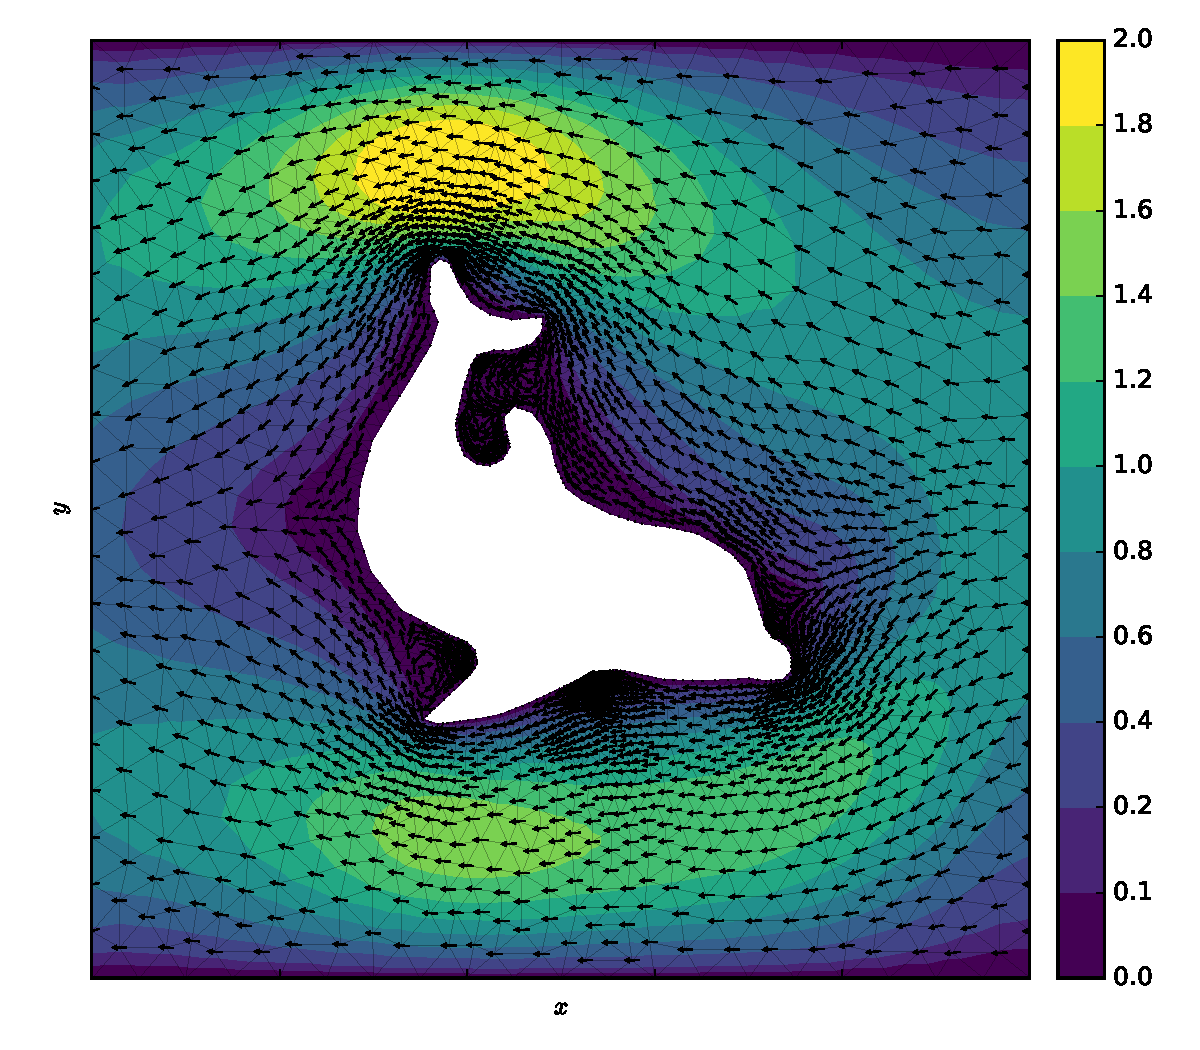
\includegraphics[width=\linewidth]{images/fenics_intro/2Dstokes_u.pdf}
  \end{minipage}
  \quad
  \begin{minipage}[b]{0.60\linewidth}
    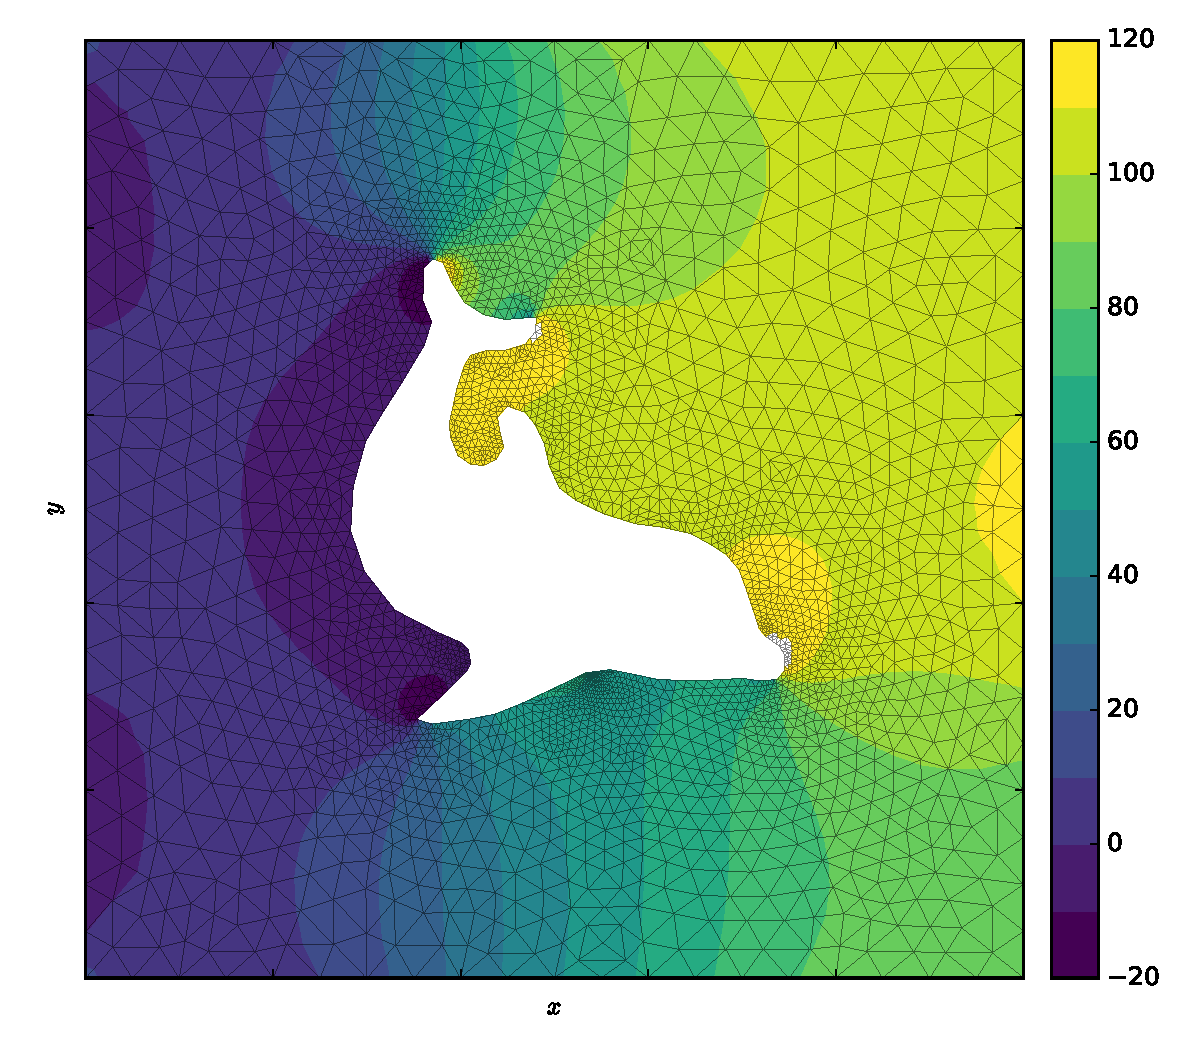
\includegraphics[width=\linewidth]{images/fenics_intro/2Dstokes_p.pdf}
  \end{minipage}
  \caption[Two-dimensional-no-slip Stokes example]{Velocity field $\rankone{u}$ (top) and pressure $p$ (bottom) for the no-slip formulation given in \S \ref{ssn_intro_stokes_2d} using the Taylor-hood element (referred to as the P2 -- P1 approximation).}
  \label{intro_stokes_2d}
\end{figure*}

\begin{figure*}
  \centering
  \begin{minipage}[b]{0.60\linewidth}
    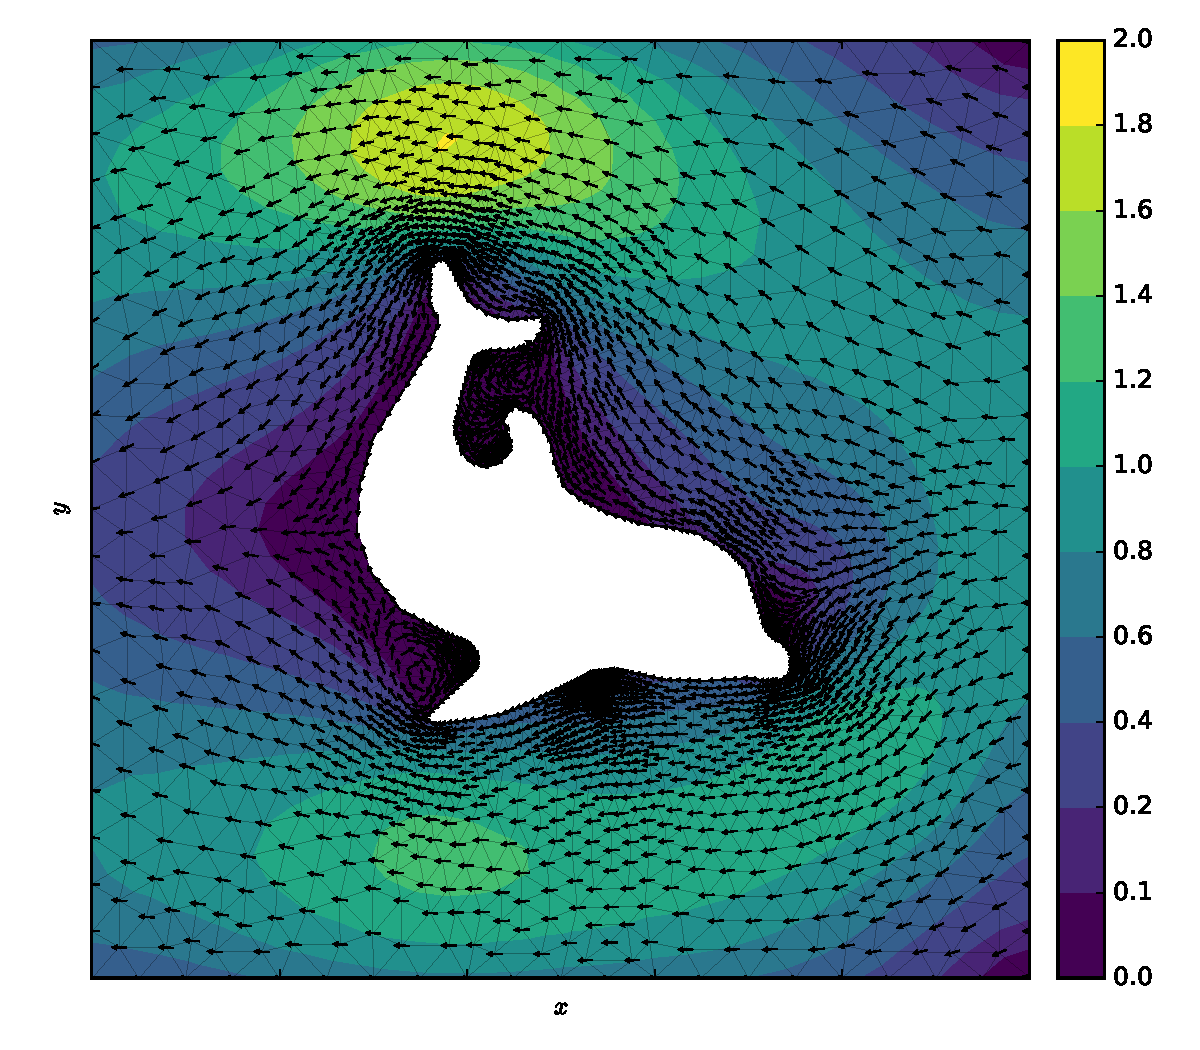
\includegraphics[width=\linewidth]{images/fenics_intro/2Dstokes_nitsche_u.pdf}
  \end{minipage}
  \quad
  \begin{minipage}[b]{0.60\linewidth}
    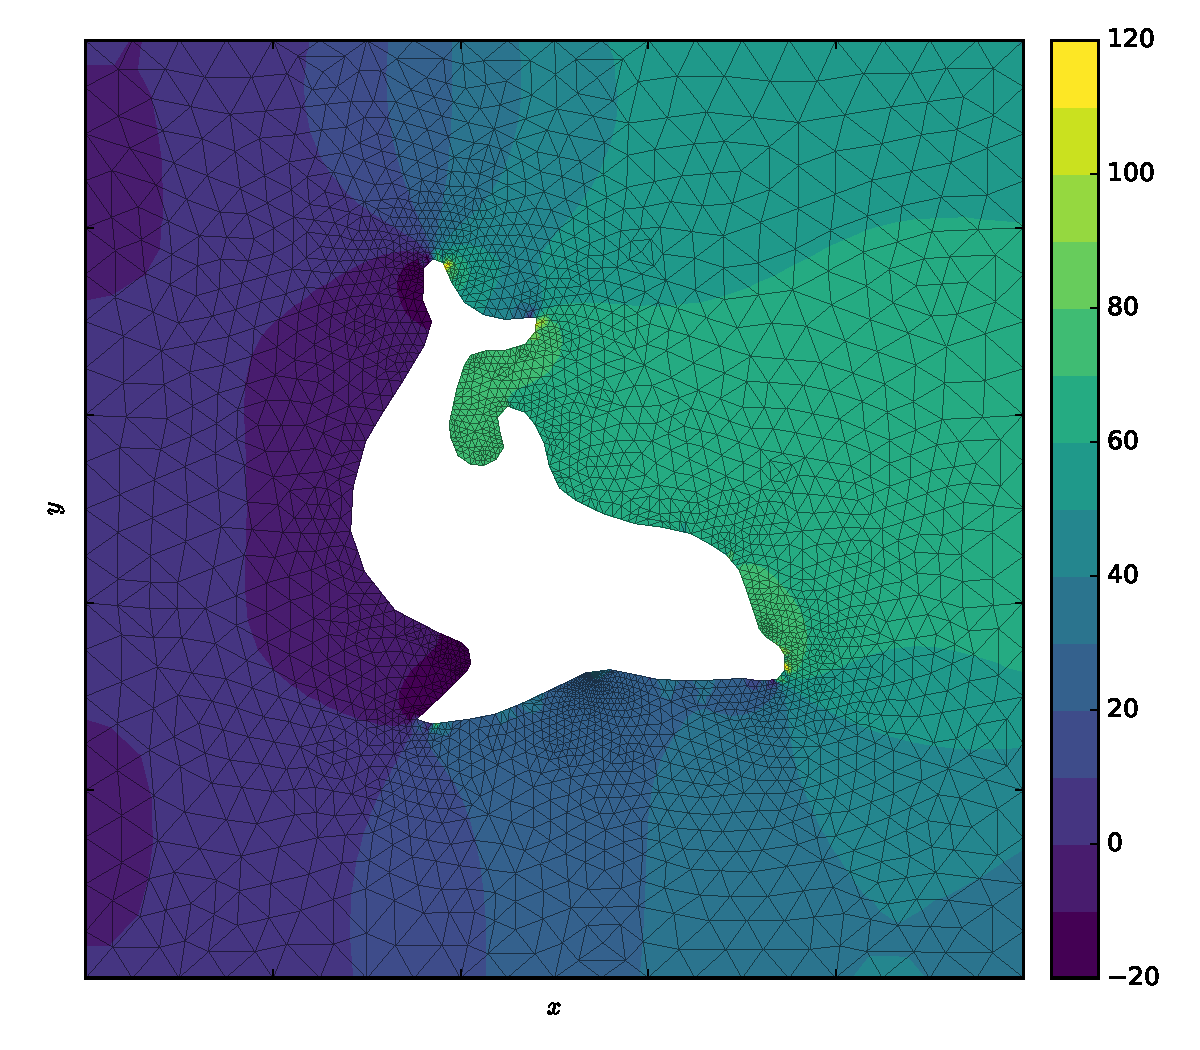
\includegraphics[width=\linewidth]{images/fenics_intro/2Dstokes_nitsche_p.pdf}
  \end{minipage}
  \caption[Two-dimensional-slip-friction Stokes example]{Velocity field $\rankone{u}$ (top) and pressure $p$ (bottom) for the slip-friction formulation given in \S \ref{ssn_intro_stokes_2d_slip} using the same Taylor-Hood element as model \S \ref{ssn_intro_stokes_2d}, with results depicted in Figure \ref{intro_stokes_2d}.}
  \label{intro_stokes_2d_nitsche}
\end{figure*}
